\documentclass[12pt,a4paper]{article}
\usepackage[a4paper,top=12mm,bottom=14mm,left=15mm,right=15mm]{geometry}
\usepackage[T1]{fontenc}
\usepackage{amsmath}
\usepackage{amssymb}
\usepackage{cancel}
\usepackage{enumitem}
\usepackage{multicol}
\usepackage{array}
\usepackage{xcolor}
\usepackage{tikz}
\usepackage[most]{tcolorbox}
\usetikzlibrary{arrows.meta,decorations.pathreplacing}

% ================================================================
% The laws of indices.
%
% A first sheet on the laws of indices for a top set Year 8 class,
% following on from the introduction to indices and roots. Each law
% is shown first by writing the powers out in full, then boxed, then
% practised in a dense list of questions: multiplying powers,
% dividing powers, zero and negative indices (met through the
% halving pattern of the powers of 2), and powers of powers. The
% laws are then used to simplify algebraic expressions with
% coefficients and more than one variable.
%
% The last part takes fractions and decimals as the base, still with
% whole-number indices only. A negative index turns the fraction
% upside down, and a decimal base is written as a simplified fraction
% first, so that the calculation only uses whole numbers. The sheet
% ends with tiles and cubes that give a negative index a meaning, and
% with open questions. Answers are on the last page.
%
% The sheet is written on, so every question is followed by a working
% area. The \newpage commands in the body are placed so that no
% question is split across a page.
% ================================================================

\pagestyle{empty}
\linespread{1.15}\selectfont
\setlength{\parskip}{5pt}
\setlist[enumerate,1]{label=\textbf{Q\arabic*.}, leftmargin=*, itemsep=10pt, topsep=6pt, parsep=4pt}
\setlist[enumerate,2]{label=(\alph*), leftmargin=*, itemsep=8pt, topsep=5pt, parsep=3pt}
\setlength{\multicolsep}{4pt}
\setlength{\parindent}{0pt}

\newcommand{\ansline}[1][2.2cm]{\underline{\hspace{#1}}}
% A short gap for a single number, sized to sit inside a line of maths.
\newcommand{\gap}{\underline{\hspace{0.7cm}}}
% A gap for a number that is written as an index, or on the top or the
% bottom of a fraction. An underline sits too low to be read as an
% index, so a faint dotted box marks where the number is written. The
% size is given in points so that the box does not shrink away when it
% is set as an index.
\newcommand{\boxgap}[1][9pt]{\tikz[baseline=-0.8pt]\draw[gray!60,densely dotted,thick]
  (0,0) rectangle (#1,#1);}

% A worked example: the method shown in full before it is practised.
% The boxes are tinted only faintly, and their title bars are pale with
% coloured text rather than solid, so that the sheet is cheap to print.
\newtcolorbox{wex}[1]{colback=blue!1,colframe=blue!45!black,boxrule=0.6pt,
  colbacktitle=blue!8,coltitle=blue!50!black,
  left=6pt,right=6pt,top=3pt,bottom=4pt,
  title={\bfseries\small Worked example: #1},fonttitle=\small,
  toptitle=1pt,bottomtitle=1pt}

% The idea the sheet is built on, stated once and boxed.
\newtcolorbox{keyidea}{colback=orange!2,colframe=orange!60!black,boxrule=0.6pt,
  left=6pt,right=6pt,top=3pt,bottom=3pt}

% A law of indices, set out so that it can be found again from
% anywhere on the sheet.
\newtcolorbox{law}[1]{colback=green!1,colframe=green!35!black,boxrule=0.9pt,
  colbacktitle=green!10,coltitle=green!30!black,
  left=8pt,right=8pt,top=3pt,bottom=3pt,
  title={\bfseries Law: #1},fonttitle=\normalsize,
  toptitle=1pt,bottomtitle=1pt}

% A warning about a mistake that is easy to make.
\newtcolorbox{warning}{colback=red!2,colframe=red!55!black,boxrule=0.6pt,
  left=6pt,right=6pt,top=3pt,bottom=3pt}

% The section headings, kept tight so the parts do not eat the page.
\newcommand{\heading}[1]{%
  \vspace{-5pt}
  {\color{blue!45!black}\rule{\linewidth}{1pt}}\\[1pt]
  {\large\bfseries #1}\\[-6pt]
  {\color{blue!45!black}\rule{\linewidth}{0.4pt}}
  \par\vspace{-6pt}}
\newcommand{\parttitle}[2]{\heading{Part #1: #2}}

% ----------------------------------------------------------------
% A row of powers above a row of their values, with an arrow between
% neighbouring values showing the division that takes one value to
% the next. \ladder{<arrow label>}{<seven powers>}{<seven values>}
% Any power or value can be left as {} for pupils to fill in.
\newcommand{\ladder}[3]{%
\begin{tikzpicture}[baseline=(current bounding box.north),
    pw/.style={draw=blue!45!black,rounded corners=2pt,thick,fill=white,
      minimum width=1.35cm,minimum height=0.75cm,inner sep=2pt},
    vl/.style={pw,draw=orange!60!black,minimum height=1cm}]
  \node[font=\small\bfseries,anchor=east] at (-0.8,0) {Power};
  \node[font=\small\bfseries,anchor=east] at (-0.8,-1.05) {Value};
  \foreach [count=\i from 0] \p in {#2} \node[pw] (p\i) at ({2.05*\i},0) {\p};
  \foreach [count=\i from 0] \v in {#3} \node[vl] (v\i) at ({2.05*\i},-1.05) {\v};
  \foreach \i [evaluate=\i as \j using int(\i+1)] in {0,...,5}
    \draw[-{Stealth},gray!70!black] (v\i.east) --
      node[above,font=\small,black,inner sep=1pt] {#1} (v\j.west);
\end{tikzpicture}}

% A square with sides of 1, split into ninths, with a square of side
% 2/3 shaded: the shaded part is (2/3)^2 = 4/9 of the whole.
\newcommand{\thirdsquare}{%
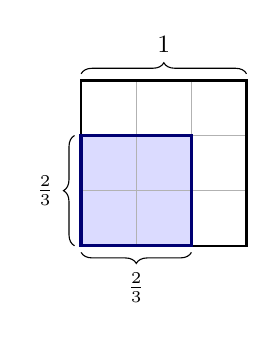
\begin{tikzpicture}[baseline=(current bounding box.north),scale=0.7]
  \fill[blue!14] (0,0) rectangle (2,2);
  \draw[gray!60] (0,0) grid (3,3);
  \draw[thick] (0,0) rectangle (3,3);
  \draw[very thick,blue!45!black] (0,0) rectangle (2,2);
  \draw[decorate,decoration={brace,mirror,amplitude=4pt}] (0,-0.12) -- (2,-0.12)
    node[midway,below=4pt,font=\small] {$\frac23$};
  \draw[decorate,decoration={brace,amplitude=4pt}] (-0.12,0) -- (-0.12,2)
    node[midway,left=4pt,font=\small] {$\frac23$};
  \draw[decorate,decoration={brace,amplitude=4pt}] (0,3.12) -- (3,3.12)
    node[midway,above=4pt,font=\small] {$1$};
\end{tikzpicture}}

% A square with sides of 1, split into hundredths, with a square of
% side 0.3 shaded: the shaded part is 0.3^2 = 9/100 of the whole.
\newcommand{\tenthsquare}{%
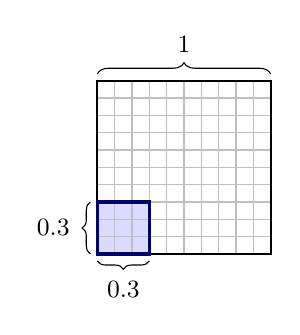
\begin{tikzpicture}[baseline=(current bounding box.north),scale=0.22]
  \fill[blue!14] (0,0) rectangle (3,3);
  \draw[gray!50] (0,0) grid (10,10);
  \draw[thick] (0,0) rectangle (10,10);
  \draw[very thick,blue!45!black] (0,0) rectangle (3,3);
  \draw[decorate,decoration={brace,mirror,amplitude=3pt}] (0,-0.4) -- (3,-0.4)
    node[midway,below=4pt,font=\small] {$0.3$};
  \draw[decorate,decoration={brace,amplitude=3pt}] (-0.4,0) -- (-0.4,3)
    node[midway,left=4pt,font=\small] {$0.3$};
  \draw[decorate,decoration={brace,amplitude=4pt}] (0,10.4) -- (10,10.4)
    node[midway,above=4pt,font=\small] {$1$};
\end{tikzpicture}}

\begin{document}
% The display skips are set here because \normalsize resets them.
\setlength{\abovedisplayskip}{3pt}\setlength{\belowdisplayskip}{3pt}
\setlength{\abovedisplayshortskip}{0pt}\setlength{\belowdisplayshortskip}{3pt}

\begin{center}
  {\Large\bfseries The Laws of Indices}
\end{center}
\vspace{-8pt}

\begin{keyidea}
In $2^5$ the number $2$ is called the \textbf{base} and the number $5$ is
called the \textbf{index}, or the \textbf{power}. The \textbf{laws of indices}
are rules for multiplying and dividing powers of the same base, and for raising
a power to another power.
\end{keyidea}

\parttitle{1}{Multiplying powers}

Writing each power out in full shows how many times the base is multiplied by
itself.
\[
2^3\times2^4=\underbrace{2\times2\times2}_{3\text{ twos}}\times
  \underbrace{2\times2\times2\times2}_{4\text{ twos}}=2^7
\]
There are $3+4=7$ twos multiplied together, so $2^3\times2^4=2^{3+4}=2^7$. A
number or a letter written without an index has an index of $1$, so $7=7^1$
and $x=x^1$.

\begin{law}{multiplying powers}
\begin{tabular}{@{}>{\large}m{3.6cm}@{\hspace{1em}}>{\raggedright\arraybackslash}m{12.8cm}@{}}
$a^m\times a^n=a^{m+n}$
  & When we multiply powers of the same base, we add the indices.\\
\end{tabular}
\end{law}

\begin{warning}
The base stays the same: $2^3\times2^4=2^7$, \textbf{not} $4^7$.
\end{warning}

\begin{enumerate}

\item Write each as a single power. Fill in the gaps in parts (a) and (b) first.
\begin{multicols}{2}
\begin{enumerate}
  \item $5^2\times5^4=5^{2+4}=5^{\boxgap}$
  \item $x^3\times x^6=x^{\boxgap+\boxgap}=x^{\boxgap}$
\end{enumerate}
\end{multicols}
\begin{multicols}{4}
\begin{enumerate}[start=3,itemsep=10pt]
  \item $3^5\times3^2=\ansline[1cm]$
  \item $10^4\times10^3=\ansline[1cm]$
  \item $7\times7^4=\ansline[1cm]$
  \item $y^2\times y^9=\ansline[1cm]$
  \item $m\times m^5=\ansline[1cm]$
  \item $a^2\times a\times a^6=\ansline[0.8cm]$
  \item $6^{\boxgap}\times6^3=6^{10}$
  \item $b^4\times b^{\boxgap}=b^{11}$
\end{enumerate}
\end{multicols}

\end{enumerate}

\parttitle{2}{Dividing powers}

We write the division as a fraction and cancel the common factors.
\[
2^5\div2^2=\frac{2\times2\times2\times\cancel{2}\times\cancel{2}}
  {\cancel{2}\times\cancel{2}}=2^3
\]
Two of the five twos cancel, which leaves $5-2=3$ twos, so
$2^5\div2^2=2^{5-2}=2^3$.

\begin{law}{dividing powers}
\begin{tabular}{@{}>{\large}m{4.6cm}@{\hspace{1em}}>{\raggedright\arraybackslash}m{11.8cm}@{}}
$a^m\div a^n=\dfrac{a^m}{a^n}=a^{m-n}$
  & When we divide powers of the same base, we subtract the indices.\\
\end{tabular}
\end{law}

\begin{enumerate}[resume]

\item Write each as a single power. Fill in the gaps in parts (a) and (b) first.
\begin{multicols}{2}
\begin{enumerate}
  \item $6^7\div6^3=6^{7-3}=6^{\boxgap}$
  \item $\dfrac{x^9}{x^4}=x^{\boxgap-\boxgap}=x^{\boxgap}$
\end{enumerate}
\end{multicols}
\begin{multicols}{4}
\begin{enumerate}[start=3,itemsep=10pt]
  \item $5^8\div5^2=\ansline[1cm]$
  \item $y^{10}\div y^3=\ansline[1cm]$
  \item $\dfrac{9^6}{9}=\ansline[1cm]$
  \item $\dfrac{a^7}{a^6}=\ansline[1cm]$
  \item $\dfrac{3^4\times3^5}{3^2}=\ansline[0.9cm]$
  \item $\dfrac{p^3\times p^8}{p^2\times p^4}=\ansline[0.8cm]$
  \item $10^{\boxgap}\div10^4=10^5$
  \item $\dfrac{b^{12}}{b^{\boxgap}}=b^3$
\end{enumerate}
\end{multicols}

\end{enumerate}

\newpage

\parttitle{3}{Zero and negative indices}

The pattern below shows powers of $2$. Each step to the right, the index goes
down by $1$ and the value is divided by $2$. Carrying on the pattern past $2^1$
shows what an index of $0$ and a negative index mean.

\vspace{2pt}
\begin{center}
\ladder{$\div2$}{$2^3$,$2^2$,$2^1$,$2^0$,$2^{-1}$,$2^{-2}$,$2^{-3}$}
  {$8$,$4$,$2$,$1$,$\frac12$,$\frac14$,$\frac18$}
\end{center}

The pattern gives $2^0=1$ and $2^{-3}=\frac18=\frac{1}{2^3}$. The law for
dividing powers gives the same results.

{\renewcommand{\arraystretch}{2.2}%
\begin{tabular}{@{}l@{\hspace{1.5em}}l@{}}
By the law, $\dfrac{2^3}{2^3}=2^{3-3}=2^0$.
  & A number divided by itself is $1$, so $\dfrac{2^3}{2^3}=1$.\\
By the law, $\dfrac{2^2}{2^5}=2^{2-5}=2^{-3}$.
  & By cancelling, $\dfrac{2^2}{2^5}
    =\dfrac{\cancel{2}\times\cancel{2}}{2\times2\times2\times\cancel{2}\times\cancel{2}}
    =\dfrac{1}{2^3}$.\\
\end{tabular}}

\begin{law}{zero and negative indices}
\renewcommand{\arraystretch}{1.6}%
\begin{tabular}{@{}>{\large}p{5.4cm}@{\hspace{1em}}l@{}}
$a^0=1$ & for example \; $7^0=1$\\
$a^{-n}=\dfrac{1}{a^n}$ & for example \; $5^{-2}=\dfrac{1}{5^2}=\dfrac{1}{25}$\\
\end{tabular}

In words: any base, except $0$, to the power $0$ is $1$. A negative index means
$1$ divided by the base to the positive index.
\end{law}

\begin{warning}
A negative index does not make the answer negative: $2^{-3}=\frac18$. It is
\textbf{not} $-8$, and it is \textbf{not} $-6$.
\end{warning}

\begin{enumerate}[resume]

\item Complete the pattern for powers of $3$.

\vspace{4pt}
\hfil\ladder{$\div3$}{$3^3$,$3^2$,{},$3^0$,{},{},$3^{-3}$}
  {$27$,$9$,{},{},$\frac13$,{},{}}\hfil

\item Work out the value of each. Give each answer as a whole number or a
fraction.
\begin{multicols}{4}
\begin{enumerate}[itemsep=16pt]
  \item $4^0=\ansline[1.2cm]$
  \item $6^{-1}=\ansline[1.2cm]$
  \item $3^{-2}=\ansline[1.2cm]$
  \item $2^{-4}=\ansline[1.2cm]$
  \item $10^{-2}=\ansline[1.2cm]$
  \item $5^{-3}=\ansline[1.2cm]$
  \item $1^{-7}=\ansline[1.2cm]$
  \item $2^{-1}+2^{-2}$\\[4pt]$=\ansline[1.2cm]$
\end{enumerate}
\end{multicols}

\end{enumerate}

\newpage

The laws of indices work in the same way with negative indices. Take care when
we subtract a negative index:
$a^3\div a^{-2}=a^{3-(-2)}=a^{3+2}=a^5$.

\begin{enumerate}[resume]

\item Write each as a single power. Fill in the gaps in parts (a) and (b) first.
\begin{multicols}{2}
\begin{enumerate}
  \item $2^{-3}\times2^5=2^{-3+5}=2^{\boxgap}$
  \item $7^2\div7^5=7^{\boxgap-\boxgap}=7^{\boxgap}$
\end{enumerate}
\end{multicols}
\begin{multicols}{4}
\begin{enumerate}[start=3,itemsep=10pt]
  \item $5^4\times5^{-6}=\ansline[0.9cm]$
  \item $x^{-2}\times x^{-3}=\ansline[0.9cm]$
  \item $3^{-2}\div3^4=\ansline[0.9cm]$
  \item $a^3\div a^{-2}=\ansline[0.9cm]$
  \item $\dfrac{y^{-4}}{y^{-6}}=\ansline[1cm]$
  \item $m^{-1}\times m=\ansline[0.9cm]$
  \item $\dfrac{4^2}{4^{-3}\times4^8}=\ansline[0.8cm]$
  \item $\dfrac{b^{-2}\times b^{-5}}{b^{-3}}=\ansline[0.8cm]$
\end{enumerate}
\end{multicols}

\end{enumerate}

\parttitle{4}{Powers of powers}

A power in a bracket raised to another power is the power in the bracket
multiplied by itself.
\[
(2^3)^4=\underbrace{2^3\times2^3\times2^3\times2^3}_{4\text{ lots of }2^3}
  =2^{3+3+3+3}=2^{12}
\]
The index $3$ is added $4$ times, which is the same as $3\times4=12$.

\begin{law}{powers of powers}
\begin{tabular}{@{}>{\large}m{3.6cm}@{\hspace{1em}}>{\raggedright\arraybackslash}m{12.8cm}@{}}
$(a^m)^n=a^{mn}$
  & When we raise a power to another power, we multiply the indices.
    Remember that $mn$ means $m\times n$.\\
\end{tabular}
\end{law}

\begin{warning}
Compare the two laws. $2^3\times2^4=2^{3+4}=2^7$ adds the indices, but
$(2^3)^4=2^{3\times4}=2^{12}$ multiplies them.
\end{warning}

\begin{enumerate}[resume]

\item Write each as a single power. Fill in the gaps in parts (a) and (b) first.
\begin{multicols}{2}
\begin{enumerate}
  \item $(5^2)^3=5^{2\times3}=5^{\boxgap}$
  \item $(x^4)^5=x^{\boxgap\times\boxgap}=x^{\boxgap}$
\end{enumerate}
\end{multicols}
\begin{multicols}{4}
\begin{enumerate}[start=3,itemsep=14pt]
  \item $(3^4)^2=\ansline[1cm]$
  \item $(y^5)^3=\ansline[1cm]$
  \item $(10^2)^{-3}=\ansline[1cm]$
  \item $(a^{-2})^{-4}=\ansline[1cm]$
  \item $(7^{-1})^5=\ansline[1cm]$
  \item $(6^3)^0=\ansline[1cm]$
  \item $(p^{\boxgap})^4=p^{12}$
  \item $(m^{-3})^{\boxgap}=m^6$
\end{enumerate}
\end{multicols}

\item \textbf{Harder.} Write each number as a single power of $2$. Remember
that $4=2^2$ and $8=2^3$.
\begin{multicols}{3}
\begin{enumerate}[itemsep=12pt]
  \item $4^3=(2^2)^3=2^{\boxgap}$
  \item $8^4=\ansline[1.3cm]$
  \item $8^2\times4^{-1}=\ansline[1.3cm]$
  \item $\dfrac{1}{32}=\ansline[1.3cm]$
  \item $16^{-2}=\ansline[1.3cm]$
  \item $\dfrac{4^5}{8^3}=\ansline[1.3cm]$
\end{enumerate}
\end{multicols}

\end{enumerate}

\newpage

\parttitle{5}{Simplifying expressions with indices}

In an expression such as $3a^2$, the number $3$ is called the
\textbf{coefficient}, and $3a^2$ means $3\times a^2$. To simplify a
multiplication or a division, we work out the coefficients using ordinary
arithmetic and use the laws of indices on each letter. Different letters are
dealt with separately.

\begin{wex}{simplifying expressions}
\small
\renewcommand{\arraystretch}{1.5}%
\begin{tabular}{@{}l@{\hspace{1.2em}}l@{}}
$3a^2\times4a^5=(3\times4)\times a^{2+5}=12a^7$
  & multiply the coefficients, add the indices\\
$12x^7\div4x^2=(12\div4)\times x^{7-2}=3x^5$
  & divide the coefficients, subtract the indices\\
$2a^3b\times5ab^4=(2\times5)\times a^{3+1}\times b^{1+4}=10a^4b^5$
  & deal with each letter separately\\
$(2y^3)^4=2^4\times y^{3\times4}=16y^{12}$
  & the $4$ applies to the coefficient as well\\
\end{tabular}
\end{wex}

\begin{warning}
In $(2y^3)^4$ the index $4$ applies to everything inside the bracket,
including the $2$. So $(2y^3)^4=16y^{12}$. It is \textbf{not} $2y^{12}$, and
it is \textbf{not} $8y^{12}$.
\end{warning}

\begin{enumerate}[resume]

\item Simplify each expression. Fill in the gaps in parts (a) and (b) first.
\begin{enumerate}
  \item $5x^3\times2x^4=(5\times2)\times x^{3+4}=\gap\,x^{\boxgap}$
  \item $18p^5\div6p^2=(\gap\div\gap)\times p^{\boxgap-\boxgap}=\ansline[1.6cm]$
\end{enumerate}
\begin{multicols}{3}
\begin{enumerate}[resume,itemsep=12pt]
  \item $4y\times3y^6=\ansline[1.6cm]$
  \item $20m^8\div5m^2=\ansline[1.6cm]$
  \item $6a^2b\times2ab^3=\ansline[1.6cm]$
  \item $\dfrac{15x^4y^5}{3xy^2}=\ansline[1.6cm]$
  \item $(3x^2)^2=\ansline[1.6cm]$
  \item $(2a^3b)^3=\ansline[1.6cm]$
  \item $3x^{-2}\times4x^5=\ansline[1.6cm]$
  \item $\dfrac{10y^3}{2y^5}=\ansline[1.6cm]$
  \item $(5k^{-1})^2=\ansline[1.6cm]$
\end{enumerate}
\end{multicols}

\item The shapes are not drawn to scale. The area of a rectangle is its length
multiplied by its width, and the volume of a cube is its edge length cubed.
\vspace{2pt}

\begin{minipage}[t]{0.32\linewidth}
\raggedright
(a) Fill in the gaps to find the area.

\vspace{4pt}
\centering
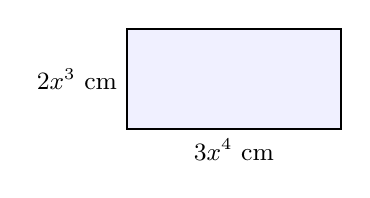
\begin{tikzpicture}[baseline=(current bounding box.north),scale=0.85]
  \draw[thick,fill=blue!6] (0,0) rectangle (3.2,1.5);
  \node[below,font=\small] at (1.6,0) {$3x^4$ cm};
  \node[left,font=\small] at (0,0.75) {$2x^3$ cm};
\end{tikzpicture}

\vspace{6pt}
\raggedright
Area $=(\gap\times\gap)\times x^{\boxgap+\boxgap}$

\vspace{6pt}
\hspace*{2.4em}$=\ansline[1.4cm]$ cm$^2$
\end{minipage}\hfill
\begin{minipage}[t]{0.32\linewidth}
\raggedright
(b) Work out the volume of the cube.

\vspace{4pt}
\centering
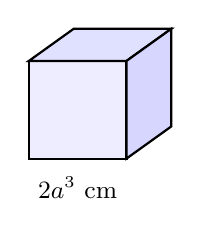
\begin{tikzpicture}[baseline=(current bounding box.north),scale=0.62,
    x={(1cm,0cm)},y={(0.46cm,0.33cm)},z={(0cm,1cm)}]
  \draw[thick,fill=blue!7]  (0,0,0)--(2,0,0)--(2,0,2)--(0,0,2)--cycle;
  \draw[thick,fill=blue!12] (0,0,2)--(2,0,2)--(2,2,2)--(0,2,2)--cycle;
  \draw[thick,fill=blue!16] (2,0,0)--(2,2,0)--(2,2,2)--(2,0,2)--cycle;
  \node[font=\small] at (1,0,-0.6) {$2a^3$ cm};
\end{tikzpicture}

\vspace{1.9em}
\raggedright
Volume $=\ansline[2cm]$ cm$^3$
\end{minipage}\hfill
\begin{minipage}[t]{0.32\linewidth}
\raggedright
(c) The area is $24x^7$ cm$^2$. Work out the length.

\vspace{4pt}
\centering
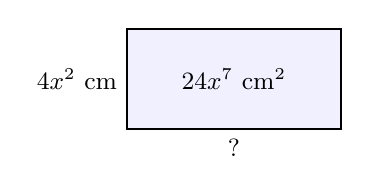
\begin{tikzpicture}[baseline=(current bounding box.north),scale=0.85]
  \draw[thick,fill=blue!6] (0,0) rectangle (3.2,1.5);
  \node[font=\small] at (1.6,0.75) {$24x^7$ cm$^2$};
  \node[below,font=\small] at (1.6,0) {$?$};
  \node[left,font=\small] at (0,0.75) {$4x^2$ cm};
\end{tikzpicture}

\vspace{3.2em}
\raggedright
Length $=\ansline[2cm]$ cm
\end{minipage}

\vspace{4pt}
\item Write down three different expressions that simplify to $16x^{12}$: one
that uses multiplication, one that uses division and one that uses a bracket.

\vspace{16pt}
\ansline[5cm]\hfill\ansline[5cm]\hfill\ansline[5cm]

\end{enumerate}

\newpage

\parttitle{6}{Fractions and decimals as the base}

When the base is a fraction, the index applies to the numerator and to the
denominator.

\begin{minipage}[t]{0.68\linewidth}
\vspace{0pt}
\[
\left(\frac23\right)^2=\frac23\times\frac23=\frac{2\times2}{3\times3}
  =\frac{2^2}{3^2}=\frac49
\]
The diagram shows a square with sides of $\frac23$ inside a square with sides
of $1$. The shaded square covers $4$ of the $9$ small squares, which is
$\frac49$ of the whole square.
\end{minipage}\hfill
\begin{minipage}[t]{0.28\linewidth}
\vspace{0pt}
\centering
\thirdsquare
\end{minipage}

\vspace{4pt}
The \textbf{reciprocal} of a fraction is the fraction turned upside down, so the
reciprocal of $\frac23$ is $\frac32$. By the law for negative indices,
\[
\left(\frac23\right)^{-2}=1\div\left(\frac23\right)^2=1\div\frac49
  =1\times\frac94=\frac94,
\]
which is the same as $\left(\frac32\right)^2$. A negative index takes the
reciprocal of the base, and then the positive index is applied.

\begin{law}{fractions as the base}
\renewcommand{\arraystretch}{2}%
\begin{tabular}{@{}>{\large}p{5.4cm}@{\hspace{1em}}l@{}}
$\left(\dfrac ab\right)^n=\dfrac{a^n}{b^n}$
  & for example \; $\left(\dfrac23\right)^2=\dfrac{2^2}{3^2}=\dfrac49$\\
$\left(\dfrac ab\right)^{-n}=\left(\dfrac ba\right)^n$
  & for example \; $\left(\dfrac23\right)^{-2}=\left(\dfrac32\right)^2=\dfrac94$\\
\end{tabular}

In words: a negative index turns the fraction upside down. Then the index is
applied to the numerator and to the denominator.
\end{law}

\begin{enumerate}[resume]

\item Work out the value of each. Give each answer as a fraction or a whole
number. Fill in the gaps in parts (a) and (b) first.
\begin{multicols}{2}
\begin{enumerate}
  \item $\left(\dfrac34\right)^2=\dfrac{3^2}{4^2}=\dfrac{\boxgap}{\boxgap}$
  \item $\left(\dfrac25\right)^{-2}=\left(\dfrac{\boxgap}{\boxgap}\right)^2
        =\dfrac{\boxgap}{\boxgap}$
\end{enumerate}
\end{multicols}
\begin{multicols}{4}
\begin{enumerate}[start=3,itemsep=12pt]
  \item $\left(\dfrac12\right)^3=\ansline[1cm]$
  \item $\left(\dfrac23\right)^3=\ansline[1cm]$
  \item $\left(\dfrac14\right)^{-1}=\ansline[1cm]$
  \item $\left(\dfrac34\right)^{-1}=\ansline[1cm]$
  \item $\left(\dfrac13\right)^{-2}=\ansline[1cm]$
  \item $\left(\dfrac23\right)^{-3}=\ansline[1cm]$
  \item $\left(\dfrac52\right)^{-2}=\ansline[1cm]$
  \item $\left(\dfrac79\right)^0=\ansline[1cm]$
\end{enumerate}
\end{multicols}

\end{enumerate}

\textbf{Decimals as the base.} A decimal base is easier to work with once it is
written as a fraction. For example, $0.3=\frac{3}{10}$, so

\begin{minipage}[t]{0.7\linewidth}
\vspace{0pt}
\[
0.3^2=\left(\frac{3}{10}\right)^2=\frac{3^2}{10^2}=\frac{9}{100}=0.09
\]
The diagram shows a square with sides of $0.3$ inside a square with sides of
$1$. The shaded square covers $9$ of the $100$ small squares.

\begin{warning}
$0.3^2=0.09$. It is \textbf{not} $0.9$, and it is \textbf{not} $0.6$.
\end{warning}
\end{minipage}\hfill
\begin{minipage}[t]{0.26\linewidth}
\vspace{0pt}
\centering
\tenthsquare
\end{minipage}

\newpage

Writing the decimal as a fraction helps most when the index is negative.
Without a calculator, $0.4^{-2}=\frac{1}{0.4^2}=\frac{1}{0.16}$, and dividing
$1$ by $0.16$ is difficult. When we write $0.4$ as a fraction first, the
calculation only uses whole numbers. We simplify the fraction before using the
index, so that the numbers stay small.

\begin{wex}{work out $0.4^{-2}$}
\small
\renewcommand{\arraystretch}{2.1}%
\begin{tabular}{@{}l@{\hspace{1.2em}}l@{}}
\textbf{Step 1 --- write the decimal as a fraction.}
  & $0.4=\dfrac{4}{10}$\\
\textbf{Step 2 --- simplify the fraction.}
  & $\dfrac{4}{10}=\dfrac25$, \; so \; $0.4^{-2}=\left(\dfrac25\right)^{-2}$\\
\textbf{Step 3 --- turn the fraction upside down.}
  & $\left(\dfrac25\right)^{-2}=\left(\dfrac52\right)^2$\\
\textbf{Step 4 --- apply the index to the top and bottom.}
  & $\left(\dfrac52\right)^2=\dfrac{5^2}{2^2}=\dfrac{25}{4}$\\
\end{tabular}
\end{wex}

\begin{enumerate}[resume]

\item Fill in the gaps in parts (a) and (b), then work out parts (c) to (l) in
the same way. Give each answer as a fraction or a whole number.
\begin{enumerate}
  \item Work out $0.6^{-2}$.

\vspace{-2pt}
{\small
\renewcommand{\arraystretch}{2.1}%
\begin{tabular}{@{}l@{\hspace{1.2em}}l@{}}
\textbf{Step 1 --- write the decimal as a fraction.}
  & $0.6=\dfrac{\boxgap}{10}$\\
\textbf{Step 2 --- simplify the fraction.}
  & $\dfrac{6}{10}=\dfrac{\boxgap}{\boxgap}$, \; so \;
    $0.6^{-2}=\left(\dfrac{\boxgap}{\boxgap}\right)^{-2}$\\
\textbf{Step 3 --- turn the fraction upside down.}
  & $\left(\dfrac{\boxgap}{\boxgap}\right)^{-2}=\left(\dfrac{\boxgap}{\boxgap}\right)^2$\\
\textbf{Step 4 --- apply the index to the top and bottom.}
  & $\left(\dfrac{\boxgap}{\boxgap}\right)^2=\dfrac{\boxgap}{\boxgap}$\\
\end{tabular}}

  \item Work out $0.25^{-3}$.

\vspace{-2pt}
{\small
\renewcommand{\arraystretch}{2.1}%
\begin{tabular}{@{}l@{\hspace{1.2em}}l@{}}
\textbf{Step 1 --- write the decimal as a fraction.}
  & $0.25=\ansline[1.2cm]$\\
\textbf{Step 2 --- simplify the fraction.}
  & $\ansline[1.2cm]$, \; so \; $0.25^{-3}=\ansline[1.6cm]$\\
\textbf{Step 3 --- turn the fraction upside down.}
  & $\ansline[4cm]$\\
\textbf{Step 4 --- apply the index to the top and bottom.}
  & $\ansline[4cm]$\\
\end{tabular}}
\end{enumerate}

\vspace{2pt}
\begin{multicols}{5}
\begin{enumerate}[resume,itemsep=4.2em]
  \item $0.3^2$
  \item $0.2^3$
  \item $0.5^{-1}$
  \item $0.5^{-3}$
  \item $0.1^{-2}$
  \item $0.2^{-2}$
  \item $1.5^2$
  \item $0.75^{-2}$
  \item $2.5^{-2}$
  \item $0.8^{-1}$
\end{enumerate}
\end{multicols}
\vspace{3.5em}

\end{enumerate}

\newpage

\begin{enumerate}[resume]

\item Use the laws of indices to write each as a single power. Then work out
its value.
\begin{multicols}{3}
\begin{enumerate}[itemsep=3.2em]
  \item $0.5^3\times0.5^{-5}$
  \item $\left(\dfrac23\right)^5\div\left(\dfrac23\right)^7$
  \item $(0.2^{-1})^2$
  \item $\dfrac{0.1^4}{0.1^7}$
  \item $0.4^{-1}\times0.4^{-1}$
  \item $(0.25^2)^{-1}$
\end{enumerate}
\end{multicols}
\vspace{2.5em}

\item The diagrams are drawn to scale.
\vspace{2pt}

\begin{minipage}[t]{0.47\linewidth}
(a) A square floor with sides of $1$ m is covered with square tiles with
sides of $0.25$ m. Each tile has an area of $0.25^2$ m$^2$, so the number of
tiles needed is $1\div0.25^2=0.25^{-2}$. Work out $0.25^{-2}$, and check your
answer by counting the tiles.

\vspace{6pt}
\centering
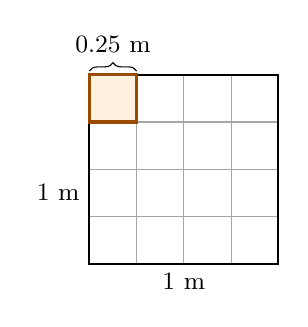
\begin{tikzpicture}[baseline=(current bounding box.north),scale=0.6]
  \fill[orange!12] (0,3) rectangle (1,4);
  \draw[gray!70] (0,0) grid (4,4);
  \draw[thick] (0,0) rectangle (4,4);
  \draw[very thick,orange!60!black] (0,3) rectangle (1,4);
  \node[below,font=\small] at (2,0) {$1$ m};
  \node[left,font=\small] at (0,1.5) {$1$ m};
  \draw[decorate,decoration={brace,amplitude=3pt}] (0,4.08) -- (1,4.08)
    node[midway,above=3pt,font=\small] {$0.25$ m};
\end{tikzpicture}

\vspace{8pt}
\raggedright
$0.25^{-2}=\ansline[5cm]$
\end{minipage}\hfill
\begin{minipage}[t]{0.47\linewidth}
(b) A crate is a cube with edges of $1$ m. It is packed with small cubes with
edges of $0.2$ m. Write the number of small cubes that fit in the crate as a
power of $0.2$, and work it out.

\vspace{6pt}
\centering
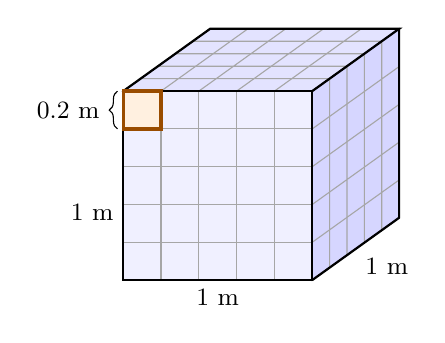
\begin{tikzpicture}[baseline=(current bounding box.north),scale=0.48,
    x={(1cm,0cm)},y={(0.46cm,0.33cm)},z={(0cm,1cm)}]
  \draw[fill=blue!6]  (0,0,0)--(5,0,0)--(5,0,5)--(0,0,5)--cycle;
  \draw[fill=blue!11] (0,0,5)--(5,0,5)--(5,5,5)--(0,5,5)--cycle;
  \draw[fill=blue!16] (5,0,0)--(5,5,0)--(5,5,5)--(5,0,5)--cycle;
  \fill[orange!12] (0,0,4)--(1,0,4)--(1,0,5)--(0,0,5)--cycle;
  \foreach \k in {1,...,4} {
    \draw[gray!70] (\k,0,0)--(\k,0,5) (0,0,\k)--(5,0,\k);
    \draw[gray!70] (\k,0,5)--(\k,5,5) (0,\k,5)--(5,\k,5);
    \draw[gray!70] (5,\k,0)--(5,\k,5) (5,0,\k)--(5,5,\k);}
  \draw[thick] (0,0,0)--(5,0,0)--(5,0,5)--(0,0,5)--cycle;
  \draw[thick] (0,0,5)--(0,5,5)--(5,5,5)--(5,0,5);
  \draw[thick] (5,0,0)--(5,5,0)--(5,5,5);
  \draw[very thick,orange!60!black] (0,0,4)--(1,0,4)--(1,0,5)--(0,0,5)--cycle;
  \draw[decorate,decoration={brace,amplitude=3pt}] (-0.15,0,4) -- (-0.15,0,5)
    node[midway,left=3pt,font=\small] {$0.2$ m};
  \node[below,font=\small] at (2.5,0,0) {$1$ m};
  \node[left,font=\small] at (0,0,1.8) {$1$ m};
  \node[below right,font=\small] at (5,2.5,0) {$1$ m};
\end{tikzpicture}

\vspace{8pt}
\raggedright
Number of small cubes $=\ansline[2.6cm]$
\end{minipage}

\vspace{6pt}
\item
\begin{enumerate}
  \item Sam says, ``$0.5^{-2}$ is a negative number, because the index is
        negative.'' Is Sam correct? Explain your answer.

\vspace{10pt}
\ansline[\linewidth]

\vspace{10pt}
\ansline[\linewidth]

  \item Write these numbers in order, from the smallest to the largest.
\[
0.5^{-3}\qquad0.2^{-2}\qquad\left(\frac32\right)^{-2}\qquad0.1^{-1}\qquad4^{-1}
\]
\vspace{4em}

  \item $16=2^4$, and $16=0.5^{-4}$. Find as many other ways as you can to
        write $16$ as a single power.
\end{enumerate}

\end{enumerate}

\newpage

\heading{Answers}

{\small
\begin{multicols}{2}
\raggedcolumns
\setlength{\parskip}{4pt}

\textbf{Q1.} (a) $5^6$ \quad (b) $x^{3+6}=x^9$ \quad (c) $3^7$ \quad
(d) $10^7$ \quad (e) $7^5$ \quad (f) $y^{11}$ \quad (g) $m^6$ \quad
(h) $a^9$ \quad (i) $7$ \quad (j) $7$

\textbf{Q2.} (a) $6^4$ \quad (b) $x^{9-4}=x^5$ \quad (c) $5^6$ \quad
(d) $y^7$ \quad (e) $9^5$ \quad (f) $a^1=a$ \quad (g) $3^7$ \quad (h) $p^5$
\quad (i) $9$ \quad (j) $9$

\textbf{Q3.} Powers: $3^3$, $3^2$, $3^1$, $3^0$, $3^{-1}$, $3^{-2}$, $3^{-3}$.
Values: $27$, $9$, $3$, $1$, $\frac13$, $\frac19$, $\frac1{27}$

\textbf{Q4.} (a) $1$ \quad (b) $\frac16$ \quad (c) $\frac19$ \quad
(d) $\frac1{16}$ \quad (e) $\frac1{100}$ \quad (f) $\frac1{125}$ \quad
(g) $1$ \quad (h) $\frac12+\frac14=\frac34$

\textbf{Q5.} (a) $2^2$ \quad (b) $7^{2-5}=7^{-3}$ \quad (c) $5^{-2}$ \quad
(d) $x^{-5}$ \quad (e) $3^{-6}$ \quad (f) $a^5$ \quad (g) $y^2$ \quad
(h) $m^0=1$ \quad (i) $4^{-3}$ \quad (j) $b^{-4}$

\textbf{Q6.} (a) $5^6$ \quad (b) $x^{4\times5}=x^{20}$ \quad (c) $3^8$ \quad
(d) $y^{15}$ \quad (e) $10^{-6}$ \quad (f) $a^8$ \quad (g) $7^{-5}$ \quad
(h) $6^0=1$ \quad (i) $3$ \quad (j) $-2$

\textbf{Q7.} (a) $2^6$ \quad (b) $(2^3)^4=2^{12}$ \quad
(c) $2^6\times2^{-2}=2^4$ \quad (d) $\frac1{2^5}=2^{-5}$ \quad
(e) $(2^4)^{-2}=2^{-8}$ \quad (f) $\frac{2^{10}}{2^9}=2^1$

\textbf{Q8.} (a) $10x^7$ \quad (b) $(18\div6)\times p^{5-2}=3p^3$ \quad
(c) $12y^7$ \quad (d) $4m^6$ \quad (e) $12a^3b^4$ \quad (f) $5x^3y^3$ \quad
(g) $9x^4$ \quad (h) $8a^9b^3$ \quad (i) $12x^3$ \quad
(j) $5y^{-2}$, or $\frac{5}{y^2}$ \quad (k) $25k^{-2}$, or $\frac{25}{k^2}$

\textbf{Q9.} (a) $(3\times2)\times x^{4+3}=6x^7$ cm$^2$ \quad
(b) $(2a^3)^3=8a^9$ cm$^3$ \quad (c) $24x^7\div4x^2=6x^5$ cm

\textbf{Q10.} Many answers. For example $4x^5\times4x^7$,
$\;32x^{15}\div2x^3$, $\;(4x^6)^2$ or $(2x^3)^4$.

\textbf{Q11.} (a) $\frac{9}{16}$ \quad (b) $\left(\frac52\right)^2=\frac{25}{4}$
\quad (c) $\frac18$ \quad (d) $\frac{8}{27}$ \quad (e) $4$ \quad
(f) $\frac43$ \quad (g) $9$ \quad (h) $\left(\frac32\right)^3=\frac{27}{8}$
\quad (i) $\left(\frac25\right)^2=\frac{4}{25}$ \quad (j) $1$

\textbf{Q12.} (a) $\frac{6}{10}$; \; $\frac35$, so
$0.6^{-2}=\left(\frac35\right)^{-2}$; \;
$\left(\frac35\right)^{-2}=\left(\frac53\right)^2$; \; $\frac{25}{9}$ \quad
(b) $\frac{25}{100}$; \; $\frac14$, so $0.25^{-3}=\left(\frac14\right)^{-3}$;
\; $\left(\frac41\right)^3=4^3$; \; $64$ \quad
(c) $\frac{9}{100}=0.09$ \quad (d) $\left(\frac15\right)^3=\frac1{125}=0.008$
\quad (e) $2$ \quad (f) $8$ \quad (g) $100$ \quad (h) $25$ \quad
(i) $\left(\frac32\right)^2=\frac94=2.25$ \quad
(j) $\left(\frac43\right)^2=\frac{16}{9}$ \quad
(k) $\left(\frac25\right)^2=\frac4{25}=0.16$ \quad (l) $\frac54=1.25$

\textbf{Q13.} (a) $0.5^{-2}=4$ \quad (b) $\left(\frac23\right)^{-2}=\frac94$
\quad (c) $0.2^{-2}=25$ \quad (d) $0.1^{-3}=1000$ \quad
(e) $0.4^{-2}=\frac{25}{4}$ \quad (f) $0.25^{-2}=16$

\textbf{Q14.} (a) $0.25^{-2}=\left(\frac14\right)^{-2}=4^2=16$ tiles \quad
(b) $1\div0.2^3=0.2^{-3}=\left(\frac15\right)^{-3}=5^3=125$ small cubes

\textbf{Q15.} (a) Sam is not correct.
$0.5^{-2}=\left(\frac12\right)^{-2}=2^2=4$, which is positive. A negative index
turns the base upside down; it does not make the value negative. \quad
(b) $4^{-1}=\frac14$, \; $\left(\frac32\right)^{-2}=\frac49$, \;
$0.5^{-3}=8$, \; $0.1^{-1}=10$, \; $0.2^{-2}=25$ \quad (c) Many answers. For
example $4^2$, $16^1$, $0.25^{-2}$, $\left(\frac14\right)^{-2}$,
$\left(\frac1{16}\right)^{-1}$, $0.0625^{-1}$, $(-4)^2$, $(-2)^4$.

\end{multicols}
}

\end{document}
